\section{Statistical Analysis System (SAS)} \label{section: SAS}
Statistical Analysis System (SAS), is a software suite for data quality, data management, and data analytics. In addition, SAS is also a programming language that is designed to be used with SAS technologies to enable data analytics.

UHTASI will be utilizing a range of SAS products suites, and analytic engines to enable data management and data analytics. This includes SAS Data Management Advanced (DMA) as the ETL solution, SAS 9.4 and SAS Visual Analytics as the runtime environments, CAS (Cloud Analytic Service) as the analytic engine, and other related SAS products that are embedded in the SAS ecosystem.

\subsection{SAS Data Management Advanced (SAS DMA)}
SAS Data Management Advanced (SAS DMA), is a software suite that provides a set of tools for data integration and data quality. The purpose of SAS DMA is to support data ETL (Extract, Transform, Load) processes, which involve extracting data from multiple sources, transforming it to meet specific requirements, and loading it into a target system for analysis and reporting. 

SAS DMA is enabled through these three components:

\begin{itemize}
    \item The \textbf{Mid-Tier} server is a web-based interface that provides access to SAS DMA workflows. This server is responsible for user authentication and authorization, job scheduling and monitoring, and other functions that are necessary for effective workflow management. It acts as a gateway for users to interact with the SAS DMA system.
    \item The \textbf{Metadata} server is responsible for managing information about data sources and workflows. It provides a central repository for storing metadata, which enables efficient management of SAS objects, definition of relationships between objects, and tracking of changes to data. In the case of SAS DMA, the metadata server manages information about data integration workflows and data quality rules.
    \item The \textbf{Compute} server provides the processing power and resources necessary to run data integration and data quality jobs. This server is responsible for executing the actual data integration and ETL tasks defined in the workflows created in SAS DMA. It ensures that the workflows are run efficiently and effectively, regardless of the size or complexity of the data being processed.
\end{itemize}

\subsection{SAS 9.4}
\href{https://documentation.sas.com/doc/en/pgmsascdc/9.4_3.5/whatsnew/n17cszme3e52b4n1ooe3710fnuec.htm#:~:text=For%20SAS%20administrators%2C%20SAS%209.4,more%20complete%20data%20management%20solution.}{SAS 9.4} is a software suite that provides tools for data management, statistical analysis, business intelligence, and predictive modeling. SAS 9.4 can handle large datasets and complex analyses by using a wide range of built-in functions and procedures that can save time and effort when working with data. 

The following software components will be integrated alongside our SAS 9.4 software suites:

\begin{itemize}
        \item Base SAS: The foundation of the SAS system and provides essential data management, analytics, and programming capabilities. It includes a powerful programming language, data manipulation tools, statistical procedures, and reporting features.
        \item Data Management Advanced Server: This component encompasses several tools for advanced data management tasks
        \begin{itemize}
            \item Data Governance - Lineage tracking and workflow management to ensure data governance and compliance.
            \item Data Quality - Data standardization, identification of duplicate records, and error detection using visual flow charts and pre-built algorithms. It aims to ensure data quality throughout the entire ETL (Extract, Transform, Load) process and can integrate smoothly with other software.
            \item Data Integration Studio - A visual interface for high-level data access, integration, and management tasks, allowing users to create visual flow charts that are converted into SAS code. It is primarily used by IT and administrators.
        \end{itemize}
        \item Enterprise Guide:  This component is designed for low to mid-level data management and access. It offers a visual interface for creating flow charts that are converted into SAS code. It is intended for use by a wide range of users, providing a user-friendly approach to data management tasks.
        \item SAS/ACCESS to MS: A component of the SAS software suite. It allows users to seamlessly access and interact with Microsoft data sources, such as Excel, Access, SQL Server, and other ODBC (Open Database Connectivity) compliant databases. This integration facilitates data extraction, transformation, and analysis using SAS tools and techniques, enhancing the interoperability between SAS and Microsoft environments.
    \end{itemize}

\subsection{SAS Visual Analytics (SAS Viya)}
SAS Visual Analytics (\href{https://documentation.sas.com/doc/en/pgmsascdc/9.4_3.5/pgmsasgswlcm/home.htm}{SAS Viya}), is a cloud-based analytics platform that provides a suite of tools and services for elastic, scalable, and fault-tolerant data analytics, data processing, and machine learning for enterprise environments. It allows organizations to store, manage, analyze, and share large volumes of data across different sources and formats.

The following software components will be integrated alongside our SAS Viya software suites:

\begin{itemize}
    \item SAS Visual Analytics: A tool for creating interactive reports and dashboards to explore and visualize data.
    \item SAS Visual Statistics: A tool for performing statistical analysis and building predictive models on large data sets.
    \item SAS Visual Data Mining and Machine Learning: A tool for exploring and analyzing large data sets using advanced analytics techniques such as clustering, decision trees, and neural networks.
    \item SAS Visual Forecasting: A tool for creating accurate and reliable forecasts using time series data.
    \item SAS In-Memory Statistics: A tool for performing high-performance analytics and modeling on large data sets using in-memory processing.
    \item Viya Platform: SAS Viya is a cloud-native and open analytics platform that provides scalable and distributed processing capabilities. It allows users to perform advanced analytics, machine learning, and data visualization tasks in a collaborative and scalable environment.
    \item Visual Text Analytics: A tool for analyzing unstructured text data, extracting insights, and uncovering patterns and sentiments within text documents.
    \item Model Manager: A component that facilitates model development, deployment, and monitoring. It enables organizations to efficiently manage and govern their analytical models throughout their lifecycle.
    \item SAS Optimization: A module that offers optimization techniques to solve complex business problems involving resource allocation, scheduling, logistics, and more. It helps organizations optimize their operations and make data-driven decisions.
    \item SAS IML (Interactive Matrix Language): A programming language within SAS that provides a flexible and interactive environment for matrix computations, statistical analysis, and modeling. It enables users to perform advanced analytics and create custom statistical models.
    \item SAS QC (Quality Control): A set of procedures and tools for statistical quality control and process improvement. It helps organizations monitor and analyze data to ensure quality standards and identify areas for improvement.
    \item SAS Econometrics: A package that provides econometric modeling and analysis capabilities. It allows users to analyze economic data, estimate models, and make predictions or forecasts based on economic relationships.
    \item Data Preparation: SAS offers various tools and techniques for data preparation, data cleaning, and transformation. These tools help users cleanse and structure their data for analysis, ensuring data accuracy and integrity.
    \item SAS/ACCESS Engines: SAS provides access engines that enable users to interact with data stored in different database management systems (DBMS). These engines allow SAS to read, write, and manipulate data in various formats and databases.
    \item Visual Analytics Add-In For Office: An integration that allows users to access and analyze SAS Visual Analytics reports directly within Microsoft Office applications, such as Excel and PowerPoint. It enables users to leverage the power of SAS analytics while working in their familiar Office environment.
\end{itemize}

To carry out these processes, SAS utilizes the Cloud Analytic Services (CAS) framework.

\subsection{Cloud Analytics Services (CAS)}
Cloud Analytics Services (\href{https://documentation.sas.com/doc/en/calcdc/3.3/calserverscas/n05000viyaservers000000admin.htm}{CAS}) is the in-memory analytics engine SAS Viya uses for both on-premise as well as cloud-service environments (e.g., AWS, Azure, GCP). CAS uses a combination of hardware and software where data management and analytics take place on either a single-machine or as a distributed server across multiple machines. In either single or distributed deployment, each machine (host, node, etc) will be assigned one of three roles: CAS Controller, CAS Backup Controller, CAS Worker.

\textbf{Analogy}
\\
In a restaurant kitchen, there exists three primary chefs. They are the (1) executive chef, (2) sous chef, and (3) station chef(s). The executive chef's primary role is to manage the kitchen and its staff whilst doing very little cooking. The sous chef's primary role is to be the right-hand to the executive chef, ready to manage the kitchen, share, or take over the responsibility of the executive chef at a moments notice. The station chef(s) merely wait for instructions from the executive chef, then executes the job they are given. 

This is the relationship of each CAS node with each other:
\begin{itemize}
    \item The CAS Controller is the executive chef managing the kitchen and its staff, delegating work.
    \item The CAS Backup Controller is the sous chef ready to take over the responsibility of the executive chef. 
    \item The CAS Worker(s) are the station chefs cooking what they are assigned to by the executive chef. 
\end{itemize}

\subsubsection{Role 1: CAS Controller}
Controller is the first role that can be assigned to a host for SAS Cloud Analytic Services. For both server architectures, single-machine and distributed, one machine must be designated as the Controller. The role of the Controller is to parse out work to each Worker host available. In other words, the Controller manages and controls the overall operation of the CAS environment. As the master node, the Controller is responsible for distributing workload among available CAS Workers, managing user sessions, and providing a secure environment for data retrieval and data storage. 

In a single-machine environment, the CAS Controller and CAS Worker roles can be performed by different processes or threads within the same operating system instance. However, we are not limited to this deployment method as it is also possible to have the CAS Controller and CAS Worker(s) virtually separated (on the same hardware) to increase the scalability of the deployment. The configuration of your architecture depends on what you need out of CAS.  

In a distributed environment, the CAS Controller is responsible for managing and controlling the CAS environment whilst the actual data processing and data analytics are performed by the CAS Worker(s).
%insert diagram%

\subsubsection{Role 2: CAS Backup Controller}
Backup Controller is the second role that can be assigned to a host for SAS Cloud Analytic Services. Although optional, the CAS Backup Controller is highly recommended in a distributed server environment. The role of the CAS Backup Controller is to act as a standby or hot-backup for the primary CAS Controller in case of a failure. Its primary purpose is to ensure that the system can continue to function in the event of a failure of the primary controller. The Backup Controller is typically set to passively monitor the primary controller for any signs of failure, such as a loss of connectivity or failure to respond to heartbeat messages. It does not actively participate in task scheduling or job execution while the primary controller is running normally. 

If the primary CAS Controller fails, the Backup Controller will take over as the primary controller and assume responsibility for managing the CAS worker nodes and scheduling tasks. In this scenario, the CAS worker nodes will send their status updates and job results to the Backup Controller instead of the failed primary controller.

In some systems, the Backup Controller can also be given jobs to execute as a CAS worker node. This can help to improve the system's overall performance by increasing the number of available processing resources. In this scenario, the Backup Controller can perform both the role of a CAS Controller and a CAS worker node.

\subsubsection{Role 3: CAS Workers}
Worker is the third role that can be assigned to a host for SAS Cloud Analytic Services. The CAS Worker is responsible for performing data processes and data analytics sent from the CAS Controller. For example, CAS Workers can perform data manipulations, transformations or computations on large/complex datasets. These computations are but not limited to: statistical analysis, machine learning models, text analysis, time series analysis, optimization, etc. Workers execute these computations using data stored on disk, in-memory, or in a distributed file system. 

In a distributed environment, one host will be assigned as your controller and any additional hosts are considered workers (optional CAS Backup Controller). Workers increase the overall computing power of your distributed-server and provides a solution for a scalable (up/down), distributed, and fault-tolerant environment for data storage and data analysis because the worker manages the storage of data/metadata across multiple nodes. The amount of CAS Workers needed to create an optimized distributed environment is highly dependant on data size, computation type, and workload.  
%insert diagram%

We can create two types of CAS configurations: a single-machine environment using symmetric multiprocessing \href{https://documentation.sas.com/doc/en/calcdc/3.3/calserverscas/n05000viyaservers000000admin.htm}{\textbf{(SMP)}}, or distributed server environment using massively parallel processing \href{https://documentation.sas.com/doc/en/calcdc/3.3/calserverscas/n05000viyaservers000000admin.htm}{\textbf{{(MPP)}}}.

\subsubsection{Symmetric Multiprocessing (SMP)}
The Symmetric multiprocessing (SMP) architecture is used when you want to run CAS on a machine or VM(VM) with multiple CPU cores. This is called shared-memory architecture because all the CPUs share the same memory. When a job is submitted to CAS in an SMP architecture, it is processed by the worker node(s) in parallel using the shared memory. The results are returned to the controller node, which sends them back to the user.

A typical SMP architecture for CAS consist of a single VM that serves as both the controller and the worker node. The number of VMs required will depend on the size of your data and the processing requirements of your workload. For example, if you have a large dataset or complex analytical workloads, you might deploy CAS on a VM with 8 or 16 CPU cores.

\begin{figure}[H]
    \centering
    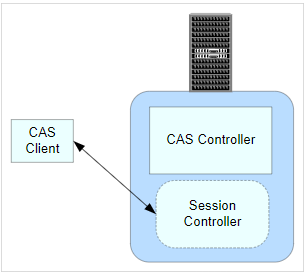
\includegraphics[scale = 0.8]{images/smp_server.png}
    \caption{\href{https://documentation.sas.com/doc/en/calcdc/3.3/calserverscas/n05000viyaservers000000admin.htm}{\textcolor{black}{Single-machine CAS Server}}}
    \label{SMP Achitecture}
\end{figure}

\subsubsection{Massively Parallel Processing (MPP)}
The Massively Parallel Processing (MPP) architecture is used when you want to run CAS on a cluster of multiple servers or VMs. This is called distributed-memory architecture because the data is partitioned and stored across multiple servers or nodes. When a job is submitted to CAS in an MPP architecture, it is distributed across the worker nodes in parallel. Each worker node processes its own subset of the data and returns the results to the controller node. The controller node then aggregates the results from all worker nodes and sends them back to the user.

A typical MPP architecture for CAS might consist of multiple VMs or servers, with some dedicated as controller nodes and others as worker nodes. The number of VMs or servers required will depend on the size of your data and the processing requirements of your workload. For example, you might choose to deploy CAS on a cluster of 10 or more VMs or servers to handle large-scale data processing tasks.

\begin{figure}[H]
    \centering
    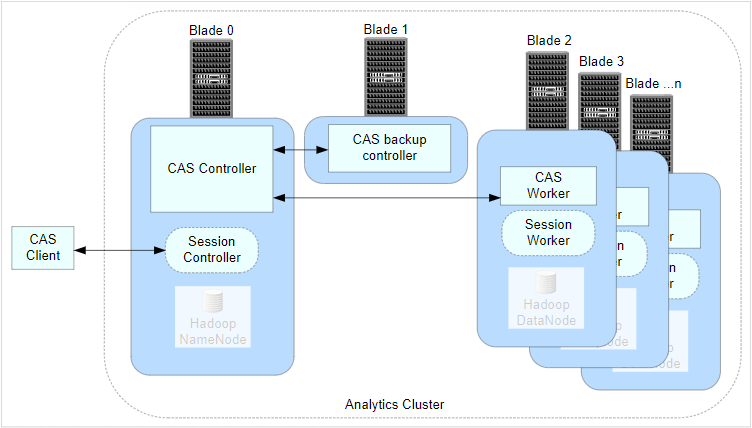
\includegraphics[scale = 0.70]{images/mpp_server.png}
    \caption{\href{https://documentation.sas.com/doc/en/calcdc/3.3/calserverscas/n05000viyaservers000000admin.htm}{\textcolor{black}{Distributed CAS Server}}}
    \label{MMP Architecture}
\end{figure}

\subsection{Algorithms \& Training}
SAS technologies offer a powerful framework for data analytics in various domains, including healthcare. With the availability of pre-built algorithms, provided by esteemed institutions such as the Centers for Disease Control and Prevention (CDC) and the Agency for Healthcare Research and Quality (AHRQ), combined with free training resources, SAS empowers organizations to effectively analyze data and derive meaningful insights, ultimately contributing to evidence-based decision-making and improved healthcare outcomes.

\subsubsection{AHRQ \& Algorithms}
The Agency for Healthcare Research and Quality (AHRQ) plays a vital role in advancing healthcare research and quality improvement initiatives. In conjunction with SAS, AHRQ offers organizations a range of pre-built algorithms or functions, developed by AHRQ's own experts, within the SAS programming language. 

These pre-built algorithms apply data analytics or conduct data quality checks on various data sources. By utilizing these algorithms, organizations can streamline their analytic processes and ensure the accuracy and reliability of their data, leading to enhanced research outcomes and more effective healthcare interventions (\href{https://qualityindicators.ahrq.gov/software/sas_qi}{SAS QI v2022}).

\subsubsection{CDC \& SAS Training}
The CDC offers comprehensive training and instruction on the SAS programming language, specifically tailored to CDC data, and this training is provided free of charge. By leveraging SAS technologies, organizations can acquire the necessary skills to effectively analyze and interpret CDC data, ultimately contributing to improved public health outcomes and evidence-based decision-making (\href{https://www.cdc.gov/std/sassi/default.htm}{SASSI}).

\subsubsection{CMS \& Packages}
The Centers for Medicare \& Medicaid Services (CMS) is responsible for administering essential healthcare programs in the United States. In collaboration with SAS, CMS provides standard libraries and packages specifically designed for data quality checks within medical-related data sources. By leveraging SAS technologies in conjunction with CMS's libraries, organizations can implement robust data quality checks to ensure the integrity and security of medical-related data (\href{https://qualitynet.cms.gov/outpatient/public-reporting/overall-ratings/sas}{Statistical Analysis System (SAS) Package}).